\section{Hiérarchie arithmétique}


Dans cette sections nous allons étudier les $\underbrace{\text{formules}}_{\land, \lor, \lnot}$
$\underbrace{\text{arithmétiques}}_{\N, +, *, \leq, \text{S}}$ du $\underbrace{\text{premier ordre}}_{\exists x, \forall x}$
sous forme prenexe et comment les classifier.


\begin{definition}[Forme prenexe]
	Une formule est sous forme prenexe si tous ses quantificateurs non bornés sont "à gauche".

	$(\forall x (x \leq 2)) \land  (\forall y (2 \leq y))$ n'est pas sous forme prenexe mais $(\forall x \forall y ((x \leq 2) \land  (2 \leq y))$ l'est.
\end{definition}



\begin{definition}
	On défini les ensembles :

	\begin{eqnarray*}
		\Sigma_{n + 1} &=& \setdef { \exists x \psi } {\psi \in \Pi_n}  \\
		\Pi_{n + 1} &=& \setdef { \forall x \psi } {\psi \in \Sigma_n}  \\
		\Delta_{n + 1} &=& \Sigma_{n + 1} \cap \Pi_{n + 1} \\
		\Delta_0 &=& \Pi_0 = \Sigma_0 \reason {formules sans quantificateurs non bornés}
	\end{eqnarray*}

	Autrement dit, $\Sigma_n$ est l'ensemble de formules avec $n$ quantificateurs alternés qui commence par un quantificateur existentiel.
\end{definition}

\begin{remarque}
	Dans la définition precedente, les formules de la forme $\forall x \forall y \ldots$ ne sont pas prises en compte. Ceci est du au fait que, grace
	au lemme suivant, les quantificateurs égaux qui se suivent peuvent être regroupés en un seul.
\end{remarque}

\begin{lemma}(Admis)
	Pour tout $\phi$ il existe $\phi_1$ et $\phi_2$ tels que :
	$$ \forall x_1, \forall x_2, \phi (x_1,x_2) \iff \forall x, \phi(\phi_1(x), \phi_2(x))$$
	Le meme résultat peut être obtenu pour le quantificateur existentiel.
	Cette propriété découle du fait que $\N \cong \N \times \N$.
\end{lemma}

\begin{prop}
	$\Delta_0$ est un ensemble calculable.
\end{prop}

\begin{proof}
	Soit $\phi \in \Delta_0$, alors, comme elle ne contient pas de quantificateurs non bornés, on peut essayer toutes les valeurs possibles, car il y a un nombre
	fini.
\end{proof}


Dans cette section nous allons étudier les relations entres ce ensembles afin de pouvoir les classifier, aboutissant a la hiérarchie de la Figure \ref{fig:arith-hier}.


\begin{figure}[h]
	\begin{center}
		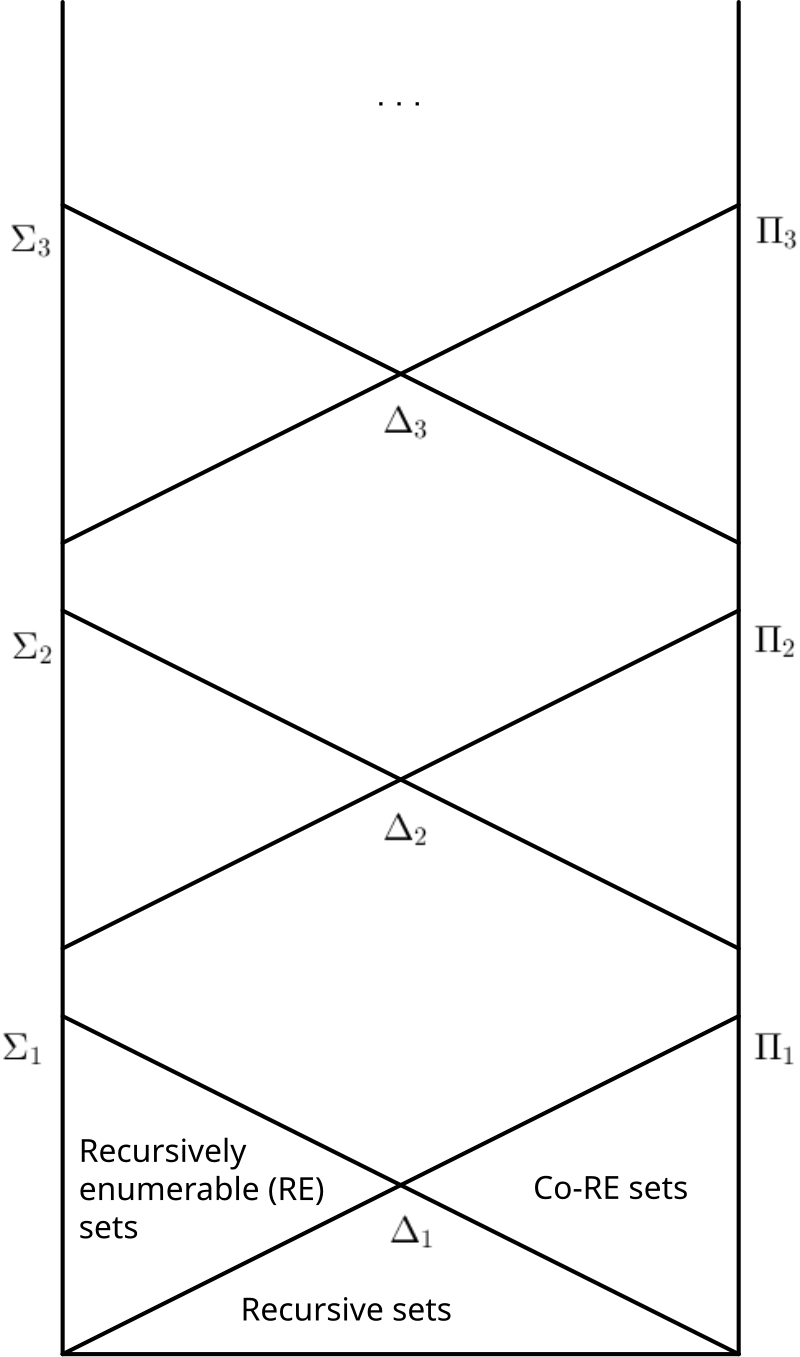
\includegraphics[height=7cm]{./images/Arithmetic_hierarchy.png}
	\end{center}
	\caption{Hiérarchie arithmétique}
	\label{fig:arith-hier}
\end{figure}


\begin{exercice}
	Montrer que $ACCEPT = \setdef {\encode {M,w}} {M(w) = 1} \in \Sigma_1$
\end{exercice}

\begin{proof}
	$$\phi (M,w) =  \exists n, \ \underbrace{eval(\encode M, w, n) = 1}_{\in \Delta_0} \in \Sigma_1$$

	Ainsi, $\phi$ décrit $ACCEPT$ et $\phi \in \Sigma_1$ et donc $ACCEPT \in \Sigma_1$.
\end{proof}


\begin{exercice}
	Montrer que $ACCEPT$ est $\Sigma_1$-complet, \ie
	$$ \forall L \in \Sigma_1, L \leqm ACCEPT $$
\end{exercice}

\begin{proof}

	Soit $L \in \Sigma_1$. Alors il existe $\phi \in \Delta_0$ \tq
	$$ L = \setdef {n} {\exists x \phi(x,n)} $$

	Soit $M(n)$ la machine qui énumere tous les $x$ et accepte si $\phi(x,n)$ est satisfaite.
	Alors $M$ reconnait $L$.
\end{proof}


\iffalse
	\begin{prop}
		$L$ est r.e. $\implies L \in \Sigma_1$.
	\end{prop}

	\begin{proof}
		\begin{eqnarray*}
			L \text{ est r.e.} &\iff& (\forall w, w \in L \iff \exists x, eval (\encode M,w,x) = 1)\\
			&\implies& L \in \Sigma_1
		\end{eqnarray*}
	\end{proof}
\fi


\begin{prop} \label{prop:sigma-re}
	$RE = \Sigma_1$
\end{prop}

\begin{proof}
	$$L \text{ est r.e.} \iff \exists L_d \text{ décidable }, L = \setdef {w} {\underbrace{\exists w', \encode {w, w'} \in L_d}_{\phi}}$$
	Et donc $RE = \Sigma_1$
\end{proof}

\subsection{Machines à oracle}

\begin{definition}[Machine de Turing à oracle]
	Une machine à oracle est une machine de Turing qui a access a une fonction $\fmots {\mathscr O}$ pendant son execution: elle a donc, en plus de la machine
	initiale, un ruban d'appel (pour l'oracle) et un état special d'appel.

	Si la machine de rentre dans l'état d'appel avec $u \in \mots$ sur le ruban, alors $\mathscr O (u) \in \mots$ est écrit sur le ruban d'appel.
\end{definition}

\begin{definition}[Reconnaissance]

	On dit que $M$ reconnait $L$ relativement a un oracle $A$ si
	$$ \forall w, M^A (w) = 1 \iff w \in L $$
	où $M^A$ est l'exécution de $M$ avec l'oracle $A$.

\end{definition}

\begin{definition}[Reduction de Turing]
	On dit que $A \leqt B \iff A$ est décidable relativement à $B$.
\end{definition}

\begin{remarque}
	On a que $A \leqm B \implies A \leqt B$ (il suffit de prendre la fonction de reduction $f$ comme l'oracle).
\end{remarque}

\begin{remarque}
	Pour tout langage $L$ on a que $L \leqt \bar L \et \bar L \leqt L$ et donc $L \equivt \bar L$.
\end{remarque}


\subsection{Hiérarchie arithmétique}

\begin{theorem}[de Post]
	Nous avons les résultats suivants :
	\begin{enumerate}
		\item \label{thm:post-1}
		      \begin{enumerate}
			      \item \label{thm:post-1a}
			            \begin{eqnarray*}
				            L \in \Sigma_{n+1} &\iff& L \text{ est r.e. relativement  un langage }  \Pi_n  \\
				            &\iff& L \text{ est r.e. relativement  un langage }  \Sigma_{n}
			            \end{eqnarray*}

			      \item
			            \begin{eqnarray*}
				            L \in \Pi_{n+1} &\iff& L \text{ est co-r.e. relativement  un langage }  \Sigma_n  \\
				            &\iff& L \text{ est co-r.e. relativement  un langage }  \Pi_n
			            \end{eqnarray*}
		      \end{enumerate}

		\item Il existe un langage $\Sigma_n$ complet, noté $\emptyset^{(n)}$. \label{thm:post-2}
	\end{enumerate}
\end{theorem}


\begin{definition}[eval avec oracle]
	$eval(\encode M, \sigma,w,t)$ évalue $M^{\sigma}(w)$ en un nombre d'étapes inférieur à $t$.
\end{definition}

\begin{proof}[Démonstration du point \ref{thm:post-1a} \bimpRL]

	$L$ est calculable relativement à $A \in \Pi_n$ via la machine $M_L$.

	\begin{eqnarray*}
		w \in L &\iff& \exists t, M^A \text{ accepte } w \text{ en un temps inférieur à } t\\
		&\iff& \exists t, \exists \sigma,
		\underbrace{\sigma \subseteq A}_{\forall u,v, (u,v) \in \sigma \ra (v=1 \iff \phi_A(u))}
		\land\  M^{\sigma} (w) \text{ accepte en temps inférieur à }t
	\end{eqnarray*}

	Ainsi, si $A \in \Pi_n$ alors $L \in \Sigma_{n+1}$. Sinon il suffit d'écrire
	$v = 0 \iff \underbrace{\lnot \phi_A(u)}_{\in \Pi_n}$ et on a aussi que $L \in \Sigma_{n+1}$.

	Les autres cas du point \ref{thm:post-1} se démontrent de manière similaire.
\end{proof}

\begin{notation}
	$\phi_{c \in \mots}$ : énumeration des fonctions calculables.

	$\phi_{c \in \mots}^X$ : énumeration des fonctions calculables relativement à $X$. Et donc $\phi_{\encode M}^X(w) = M^X(w)$
\end{notation}

\begin{definition}[Saut de Turing]
	Soit $X$ un langage,

	$X' = \setdef c {\phi_c^X(c) \text{ est défini}} = \setdef {\encode M} {M^X \text{ s'arrete sur } \encode M}$

\end{definition}

\begin{definition}
	$$\emptyset' = \setdef {\encode M} {M^{\emptyset} \text{ s'arrete sur } \encode M}$$
	$$\emptyset^{(n+1)} = \setdef {\encode M} {M^{\emptyset^{(n)}} \text{ s'arrete sur } \encode M} $$
\end{definition}


\begin{remarque}
	$$\emptyset' \equivm \halt$$
\end{remarque}

\begin{exercice}
	Montrer que $\emptyset '$ est $\Sigma_1$-complet :
	\begin{enumerate}
		\item $\emptyset' \in \Sigma_1$
		\item $\forall L \in \Sigma_1, L \leqm \emptyset'$
	\end{enumerate}
\end{exercice}

\begin{proof}
	\begin{enumerate}
		\item $\encode M \in \emptyset' \iff \exists t, eval (\encode M, ((_,0), \ldots, (_,0)), \encode M, t) \neq \bot$
		\item On a que $\emptyset' \equivm \halt$ qui est $\Sigma_1$-complet, donc $\emptyset'$ l'est aussi.
	\end{enumerate}
\end{proof}


\begin{lemma} \label{lem:trans-turing}
	Si $A$ est $C$-complet et $Y \in C$, alors :
	$$X \text{ est } re(Y) \iff X \text{ est } re(A)$$
\end{lemma}

\begin{proof}
	TODO
\end{proof}


\begin{proof}[Démonstration du point \ref{thm:post-2}]
	Il faut donc monter que $\forall n, \emptyset^{(n)}$ est $\Sigma_n$-complet.
	La demonstration est faite par induction. Les cas $n =0$ et $n=1$ on été traités precedent, il suffit alors de montrer le cas d'induction.

	Supposons $\emptyset^{(n)} \ \Sigma_n$-complet.

	\begin{eqnarray*}
		L \in \Sigma_{n+1} &\iff& \exists A \in \Sigma_n, L \text { est r.e. relativement à } A \\
		&\iff& L \text{ est re}(\emptyset^{(n)})\\
		&\iff& \exists M_L, M_L^{\emptyset^{(n)}} \text { reconnait } L \\
		&\iff^? & L \leqm \emptyset^{(n + 1)}
	\end{eqnarray*}

	\begin{itemize}
		\item \bimpLR
		      \begin{eqnarray*}
			      w \in  L  &\iff&  M_L^{\emptyset^{(n)}}(w) \text{ s'arrête et accepte} \\
			      &\iff&  M_{L,w}^{\emptyset^{(n)}}(\cdot) \text{ s'arrête } \\
			      &\iff&  \encode{M_L,w} \in \emptyset^{(n+1)} \\
			      &\iff&  L \leqm  \emptyset^{(n+1)}
		      \end{eqnarray*}
		\item \bimpRL \\
		      Comme $\emptyset^{(n+1)}$ est $re(\emptyset^{(n)})$ et $L \leqm \emptyset^{(n+1)}$ en applicant le lemme \ref{lem:trans-turing}
		      on obtient que $L$ est $re(\emptyset^{(n))}$ et donc que $\exists M_L, M_L^{\emptyset^{(n)}} \text { reconnait } L$.
	\end{itemize}
\end{proof}



On s'intéresse maintenant à savoir si la hiérarchie est stricte, \ie, $\exists \phi \in \Sigma_{n+1}, \text{ \tq }, \phi \notin \Sigma_n \et \phi \notin \Pi_n$.


\begin{prop}
	$$\forall n, \emptyset^{(n)} \notin \Delta_n$$
\end{prop}


\begin{remarque}
	Pour $n > 0$
	\begin{eqnarray*}
		L \in \Delta_n &\iff& L \in \Sigma_n \land L \in \Pi_n \\
		&\iff& L \text{ est } re(\Sigma_{n-1}) \land L \text{ est } co-re(\Sigma_{n-1})\\
		&\iff& L \text{ est } re \text{ relativement à } \emptyset^{(n-1)} \land  L \text{ est } co-re \text{ relativement à } \emptyset^{(n-1)} \\
		&\iff& L \text{ est décidable relativement à } \emptyset^{(n-1)}
	\end{eqnarray*}
\end{remarque}

\begin{proof}
	On traite d'abord le cas $n = 0$ qui est trivial car $\Delta_0 = \emptyset$.

	En suite pour $n > 0$ on peut utiliser la remarque precedente. Ainsi, il suffit de montrer que $\emptyset^{(n)}$ n'est pas décidable relativement à $\emptyset^{(n-1)}$.

	Supposons par l'absurde que $\emptyset^{(n)}$ est décidable relativement à $\emptyset^{(n-1)}$, \ie, il existe $M_n$ telle que $M_n^{\emptyset^{(n-1)}}$ décide $\emptyset^{(n)}$.

	Alors on construit

	$$
		M_0(\encode M) =
		\left\{
		\begin{array}{ll}
			\text{Si } M_n^A(\encode M) \text{ accepte} & \rightarrow \text{ boucle}  \\
			\text{Si } M_n^A(\encode M) \text{ rejecte} & \rightarrow \text{ accepte} \\
		\end{array}
		\right.
	$$

	Alors on a que
	\begin{eqnarray*}
		M_0^{\emptyset^{(n-1)}}(\encode{M_0}) \text{ boucle} &\iff& M_n^{\emptyset^{(n-1)}} (\encode {M_0}) \text{ accepte} \\
		&\iff& M_0^{\emptyset^{(n-1)}}(\encode{M_0}) \text{ s'arrête} \contradict
	\end{eqnarray*}
\end{proof}


\begin{coro}
	La hiérarchie ne s'effondre pas.
\end{coro}
